\documentclass[tikz,border=5pt]{standalone}
\usepackage{circuitikz}
\usetikzlibrary{arrows.meta,positioning,calc}

\begin{document}
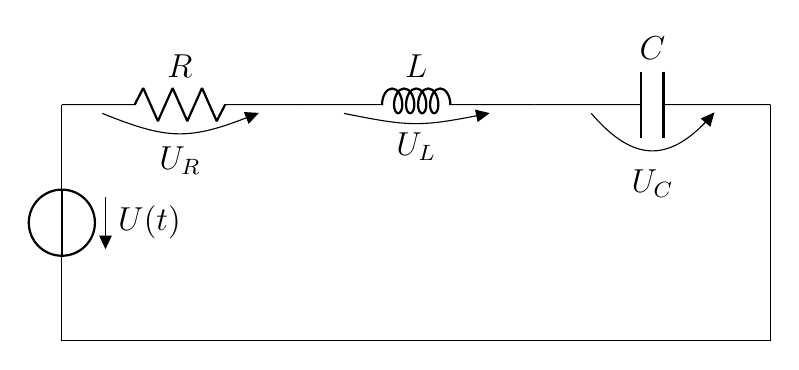
\begin{tikzpicture}[
  font=\large,
  every node/.style={font=\large}
]
  % RLC series circuit: voltage source -> R -> L -> C -> back
  % Nodes
  \coordinate (A) at (0,0);
  \coordinate (B) at (0,3);
  \coordinate (C) at (3,3);
  \coordinate (D) at (6,3);
  \coordinate (E) at (9,3);
  \coordinate (F) at (9,0);

  % Voltage source: draw from B (top) to A (bottom) without invert
  % => + at B (FROM-node, top), v-arrow points toward A (downward)
  % => matches KVL U(t) - U_R - U_L - U_C = 0
  \draw (B) to[V, v=$U(t)$] (A);

  % Top wire: R then L then C
  \draw (B) to[R, l=$R$, v=$U_R$] (C);
  \draw (C) to[L, l=$L$, v=$U_L$] (D);
  \draw (D) to[C, l=$C$, v=$U_C$] (E);

  % Return path: right side down, then along the bottom back to the source
  \draw (E) -- (F) -- (A);

\end{tikzpicture}
\end{document}

